\hypertarget{stereo-cameras}{%
\section{Stereo Cameras}\label{stereo-cameras}}

We can build cameras that are much more accurate than the eye, however,
understanding that the image belongs to a particular object is a much
harder task. Implicit in the process is our stereo vision. We have the
ability to reconstruct the 3D world through our eyes; an ability for
which significant effort has been expended to duplicate in computer
science. A branch of modern computer vision, stereo vision, uses
multiple cameras and algorithms to reconstruct and understand the
environment. Some of the tools developed to do this have been widely
distributed. For example, the automatic stitching of images that cameras
perform when building panoramas.

This is successfully employed using pairs of cameras which do a good job
at reconstructing the 3D world we live in. The process requires one to
determine the position shift in pixels of a fixed object. The difficult
part is automatically identifying common points in the image.
Significant effort has been invested in the determination of common
features between two images. Several well known algorithms such as SIFT
and SURF are available now to simplify this process. Once that is done,
it is easy to triangulate the depth of the point,
\texttt{intro-stereo1}.

\begin{quote}
Seeing in three dimensions with a pair of calibrated cameras:
determining depth using basic Trigonometry.
\end{quote}

\begin{figure}
\centering
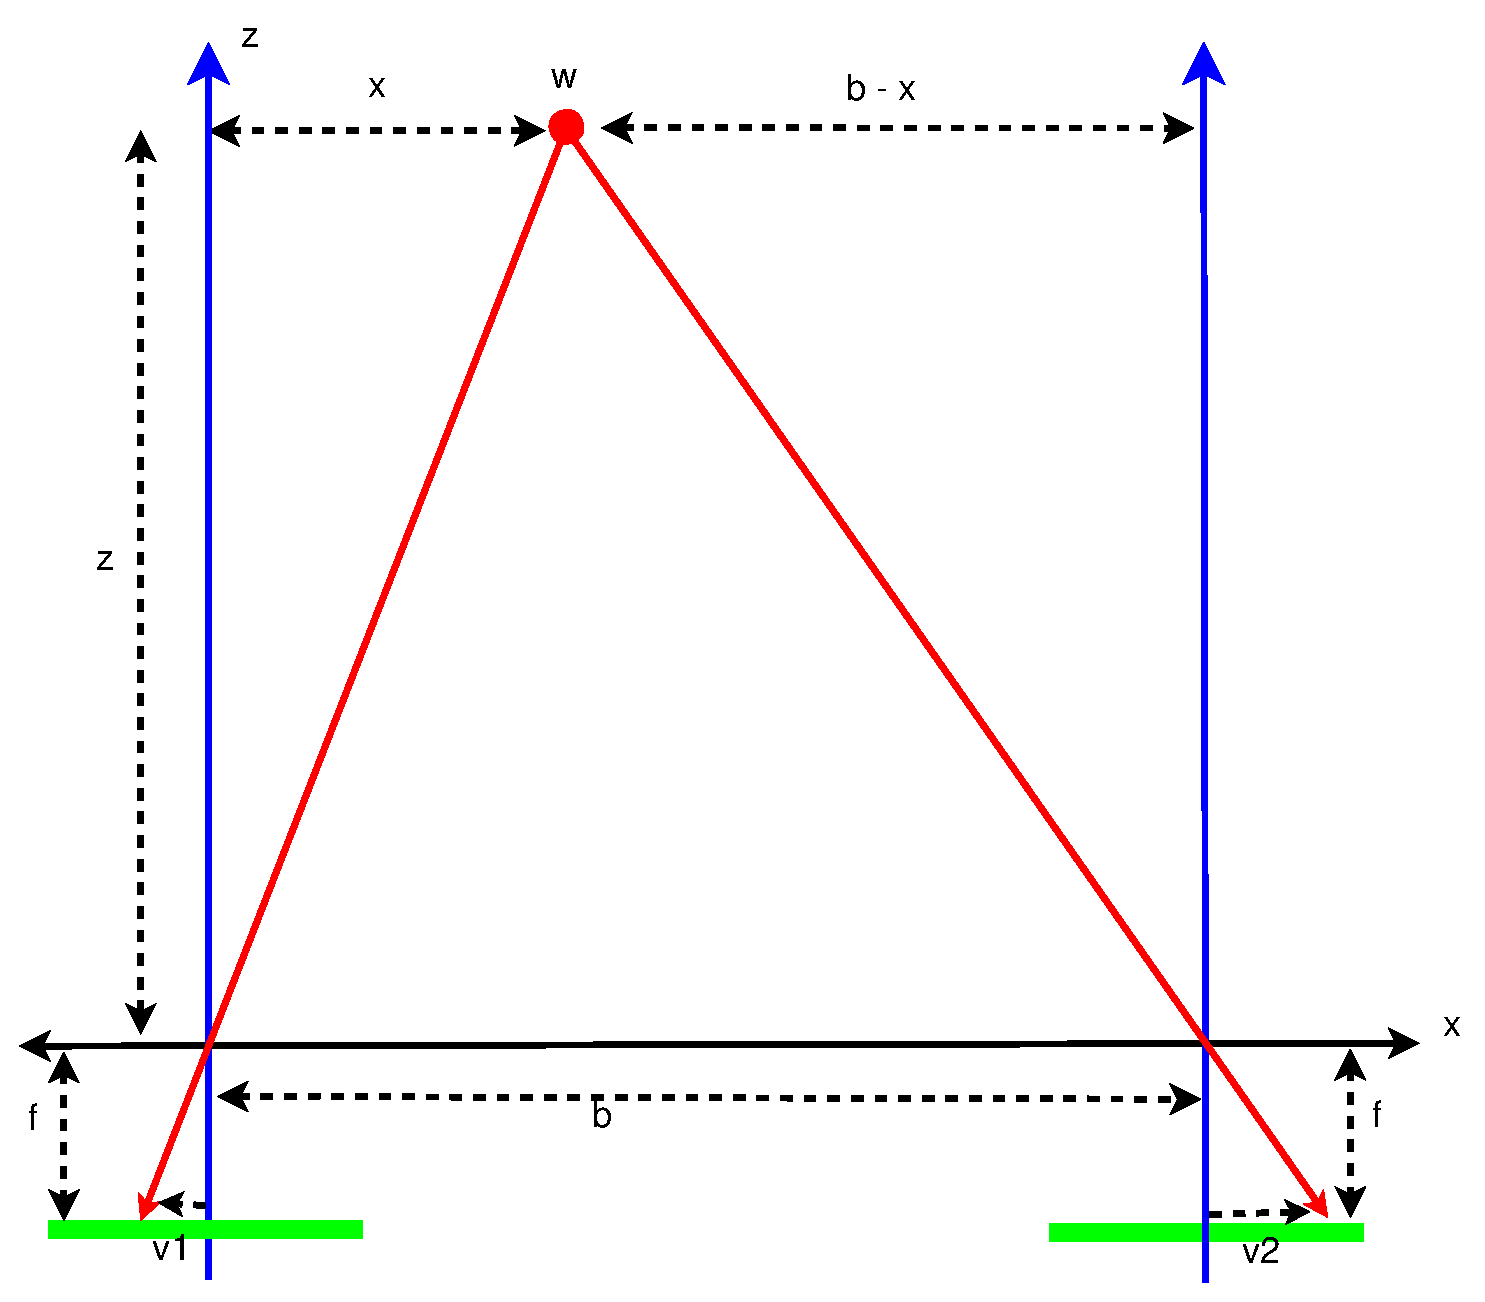
\includegraphics[width=0.5\textwidth,height=\textheight]{VisionFigures/stereo1a.*}
\caption{Seeing in three dimensions with a pair of calibrated cameras:
determining depth using basic Trigonometry.}
\end{figure}

Define a coordinate system where the horizontal axis is \(x\) and the
vertical axis is \(z\). Let the focal point of the left camera be at the
origin of the \(x-z\) coordinate system. Using both cameras, we would
like to find the coordinates \((x,z)\) for the point \(w\). Assume that
we are given the focal depth \(f\) (positive value) and pixel offsets in
image sensor \(v_1\), \(v_2\) all as \emph{unsigned} (positive)
quantities. Then

\[\left(\frac{z}{x}\right) = \left(\frac{f}{v_1}\right),\quad\quad
\left(\frac{z}{b-x}\right)  = \left(\frac{f}{v_2}\right)\]

Cross multiply and set equal to common fraction; then remove fractions:

\[\left(\frac{v_1}{x}\right) = \left(\frac{f}{z}\right) = \left(\frac{v_2}{b-x}\right)
\quad \Rightarrow \quad v_2 x = v_1(b-x) = v_1 b - v_1 x \Rightarrow  (v_1+v_2) x = v_1b\]

Solving for \(x\), we obtain the equation below. Plugging this into
\(z = fx / v_1\) we obtain the equation for \(z\).

\[x = \frac{v_1b}{v_1+v_2}, \quad
z = \frac{fb}{v_1+v_2}\]\[Seeing in three dimensions with a pair of calibrated cameras: building
a disparity (depth) map.\]\[Seeing in three dimensions with a pair of calibrated cameras:
reconstructing the 3D world.\]

Once depth for the collection of feature points are known, depth for
surrounding points is inferred. This allows the construction of a
disparity map which maps grey scale values to pixel. It is a depth map
which is shown in \texttt{fig:seeing3d-a}. A depth map is a useful tool
in object identification. The depth map can be used for segmentation,
the process by which we separate an image into distinct components or
objects. Once we have the object segmented, then we may lookup in a
shape database to determine what the object is, known as object
recognition. The depth map is one of several ways to perform object
recognition and is a useful tool if we have already computed the depth
map.

\begin{quote}
Seeing in three dimensions with RGBD sensors.
\end{quote}

Once a depth map is made, reconstruction of the environment can follow.
Essentially a 3D CAD type representation of the world surrounding the
robot. Thus the environment is mapped in 3D. This is useful for robots
which perform remote reconnaissance as well as for robots which need to
navigate through the environment according to some plan. The map
building process normally places the robot in the map, known as
localization. Thus we can compute optimal paths and safe trajectories.

\hypertarget{depth-sensing-cameras}{%
\subsection{Depth Sensing Cameras}\label{depth-sensing-cameras}}

We also have a choice of sensors which can directly measure the depth of
field. These are known as time of flight cameras or 3D cameras. The
Microsoft Kinect is a common example. The units range significantly in
cost depending on accuracy, range and speed of the device. These devices
directly provide depth without having to compute a disparity map or some
other intermediate data set. They are very helpful in doing 3D
reconstructions of the environment.

\begin{figure}
\centering
\includegraphics[width=0.5\textwidth,height=\textheight]{VisionFigures/3dcamera.*}
\caption{3D Camera}
\end{figure}
